% Course: AIM3
% Autors: Anil Pala, Franziska Adler
% Datum: 03.02.2015

\documentclass[a0,portrait]{a0poster}

\usepackage{anyfontsize}%for changing fontsize
\usepackage[ansinew]{inputenc}
\usepackage[T1]{fontenc}
\usepackage[english,ngerman]{babel}
\usepackage{amsmath} 
\usepackage{fancybox}
\usepackage{graphicx}
\unitlength1cm %picture environment 1 cm

%colums and boxes
\usepackage{multicol}
\setlength{\fboxrule}{1.50mm} %lines
\setlength{\fboxsep}{10mm} %margin text relation
\setlength{\columnsep}{15mm}     %colum space
\setlength{\columnseprule}{4pt}  % lines between columns

%page settings
\renewcommand\baselinestretch{1.35}
\parskip=0.5\baselineskip
\topmargin-30pt
\marginparwidth0mm
\oddsidemargin-20pt
\evensidemargin-20pt
\textwidth770mm
\textheight1140mm

% color
\usepackage{xcolor}
\usepackage{color} 
\definecolor{darkgreen}{rgb}{0,0.4,0.2} 
\definecolor{darkblue}{rgb}{0,0,0.5}
\definecolor{darkred}{rgb}{0.6,0,0.05}

\begin{document}
\pagecolor[rgb]{0.9,0.925,0.9}
% header
 \begin{center}
    {\huge \textbf{\\A Comparison of Online learning Na\"ive Bayes Classifier\\ on RSS Feeds using SPARK\\}}
 %   \vspace*{0.018\textheight}
  \end{center}
\begin{minipage}{0.4\textwidth}
\begin{flushleft} \large
\textbf{\emph{Authors:}\\
Anil \textsc{Pala} \& Franziska \textsc{Adler}}\\
%anil@pala.com \hspace{0.5cm} adler.franziska@gmx.de
\end{flushleft}
\end{minipage}
\hfill
\begin{minipage}{0.4\textwidth}
\begin{flushright} \large
\textbf{\textsc{\color{darkred} \Large TU Berlin}\\
Advanced Information Management III\\
Scalable Data Analytics and Data Mining}
\end{flushright}
\end{minipage}
\newcommand{\HRule}{\rule[-10mm]{805mm}{1mm}} \HRule \\[0.5cm] %line

%create first Box
\fcolorbox{darkgreen}{white}{\parbox{\textwidth}{%

    \begin{multicols}{2}      
      \begin{center} \textbf{\huge Motivation \& Problem Statement} \end{center}
Many practical applications rely on immediate data. The need for solutions to continuously conduct analyses as mathematical computations on large data amounts led to new technologies in the past years. Stream processing operates on real-time data for example through stream windowing and analytical operations within those. Since data distributions might not remain static over time a precomputed (batch) model for analysis can produce poorly results after some time [1]. The reconstruction or updating of the underlying analytical model to receive accurate results is required. This problem is known as Concept Drift. In this project we are using unstructured streaming data from BBC RSS feeds in order to classify them to their corresponding category. We focus on the evaluation of a Na\"ive Bayes Classifier with different model-update approaches to compare their analytical performance according to Concept Drift. 

    %  \begin{center} \textbf{\huge Background} \end{center}

some background stuff like how naive bayes works, concept drift, stuff some background stuff like how naive bayes works, concept drift, stuff some background stuff like how naive bayes works, concept drift, stuff some background stuff like how naive bayes works, concept drift, stuff some background stuff like how naive bayes works, concept drift, stuff some background stuff like how naive bayes works, concept drift, stuff some background stuff like how naive bayes works, concept drift, stuff some background stuff like how naive bayes works, concept drift, stuff some background stuff like how naive bayes works, concept drift, stuff some background stuff like how naive bayes works, concept drift, stuff some background stuff like how naive bayes works, concept drift, stuff some background stuff like how naive bayes works, concept drift, stuff some background stuff like how naive bayes works, concept drift, stuff some background stuff like how naive bayes works, concept 
 
    \end{multicols}}}

\vspace{0.8cm}
%create second Box
\fcolorbox{darkgreen}{white}{\parbox{\textwidth}{%

    \begin{multicols}{3}      
      \begin{center} \textbf{\huge Batch Model} \end{center}
Very sophisticated stuff.Very sophisticated stuff.Very sophisticated stuff. Very sophisticated stuff.

      \begin{center} \textbf{\huge Bruteforce Model} \end{center}
Very sophisticated stuff.Very sophisticated stuff.Very sophisticated stuff.Very sophisticated stuff.
 
      \begin{center} \textbf{\huge Incremental Model} \end{center}
In the incremental model, unlike the other update models, following an initial training-only phase, all the incoming stream items are always used for training right after the prediction. So, this way the immidiate information whether the prediction was good or bad can be used for improving the model on the fly. In other words, predictive model building and testin phases perfectly overlap in incremental model update method. We used this to achieve a real-time response to the changes in the data arguably making the text mining application more resillant to the conceptual drifts. The initial traing size of 600 is used for this model update method. 
    \end{multicols}}}

\vspace{0.8cm}
%create third Box
\fcolorbox{darkgreen}{white}{\parbox{0.4775 \textwidth}{%
      \begin{center} \textbf{\huge Data \& Setup} \end{center}
For our evaluation purposes of classifing streamed textdata we are using RSS feeds from BCC. A RSS feed is a collection of tags in xml structure which contains tags for title, a description and an url among other tags. Those listed are used in our applicaton. Our data points are constructed from title and description of the feed, the url gives us the respective label.\\
setup   


}}
\hspace{0.8cm}
%create 4. Box
\fcolorbox{darkgreen}{white}{\parbox{0.4775 \textwidth}{%
      \begin{center} \textbf{\huge Streaming} \end{center}
In order to deal with the continuos nature of the data, traditional programming primitives are not of much help. In order to make programmers's job easier, libraries providing higher lever abstractions are introduced. Knowing that, for a news feed classifier we need to split the 'main' stream into multiple streams to treat different portions of stream differently. For example, there needs to be at least two channels of streams branching out from the main one having the test items and training items. The main flow of the streaming logic we used is depicted in the figure.[2]\\
\begin{center}
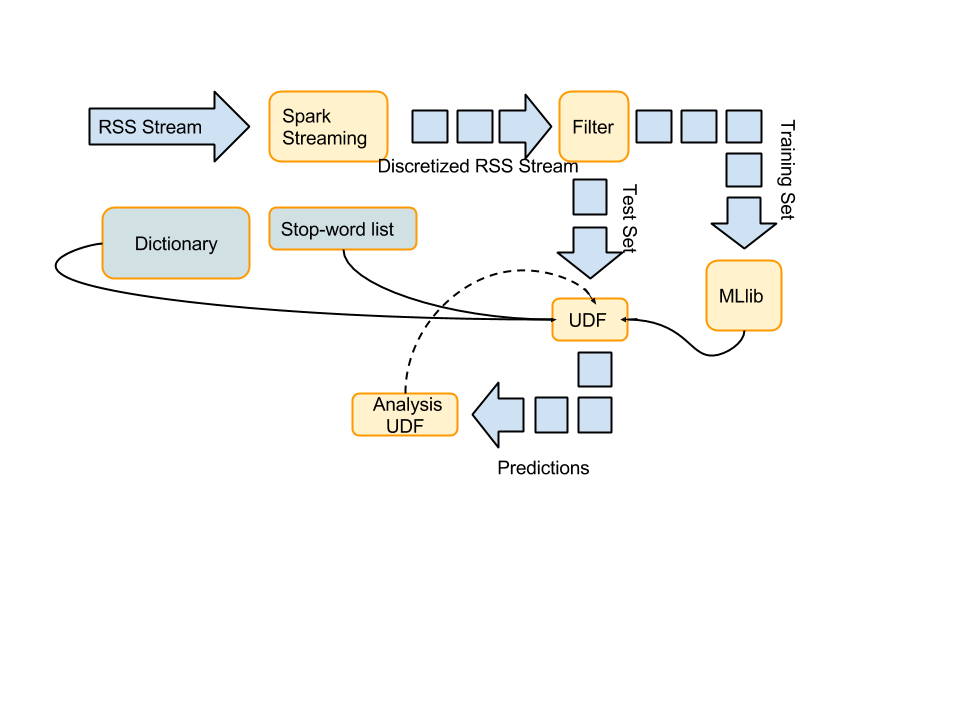
\includegraphics[width=0.2\textwidth]{./time_models/streaming_diagram}
\end{center}
}}
\hspace{0.8cm}


\vspace{0.8cm}
%create 5. Box
\fcolorbox{darkgreen}{white}{\parbox{0.4775 \textwidth}{%
\begin{centering}
      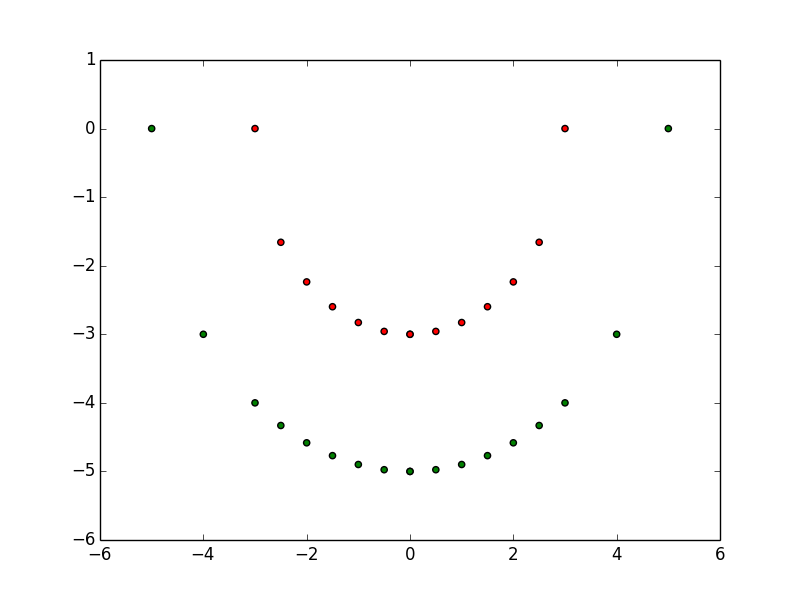
\includegraphics[width=0.2\textwidth]{./pic1}\\
Some picture with stuff
\end{centering}
 %     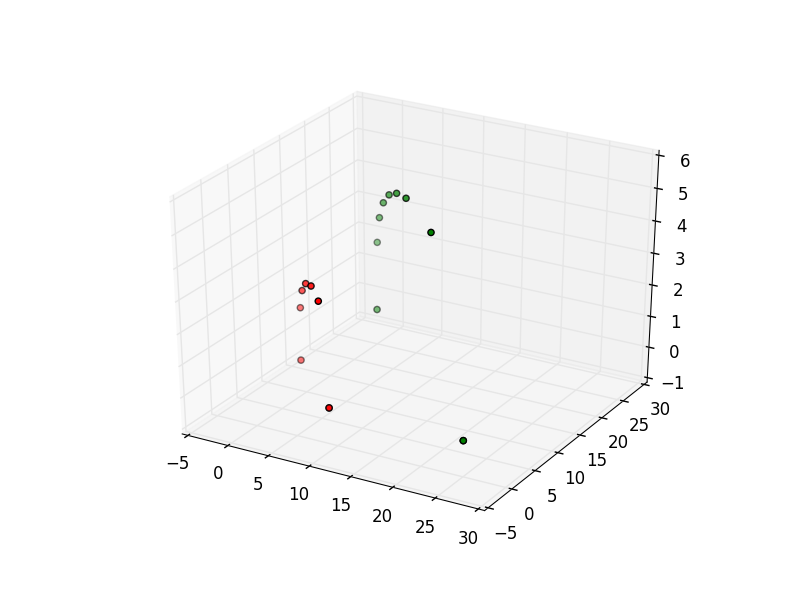
\includegraphics[width=0.15\textwidth]{./pic2}
}}
\hspace{0.8cm}
%create 6. Box
\fcolorbox{darkgreen}{white}{\parbox{0.4775 \textwidth}{%
\begin{centering}
   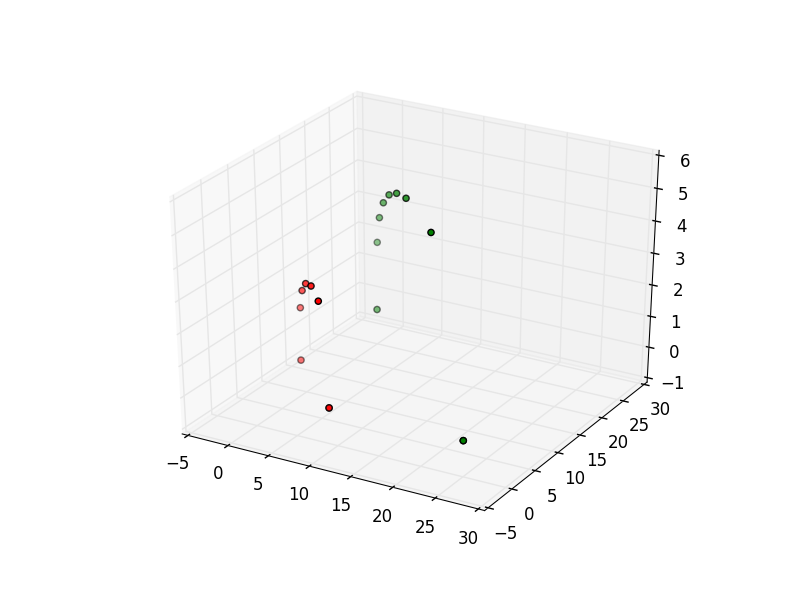
\includegraphics[width=0.2\textwidth]{./pic2}\\
some other graphic
\end{centering}}}

\vspace{0.8cm}
%create 7. Box
\fcolorbox{darkgreen}{white}{\parbox{\textwidth}{%
   \begin{center} \textbf{\huge Results} \end{center}
To evaluate the performance of our classification approaches we used the cumulative accurency per interval and the cumulative accurancy over all points which are at this time not in the training set. The batch/ offline szenario performs similar the first two test phase with but seams decreasing in the last interval.

 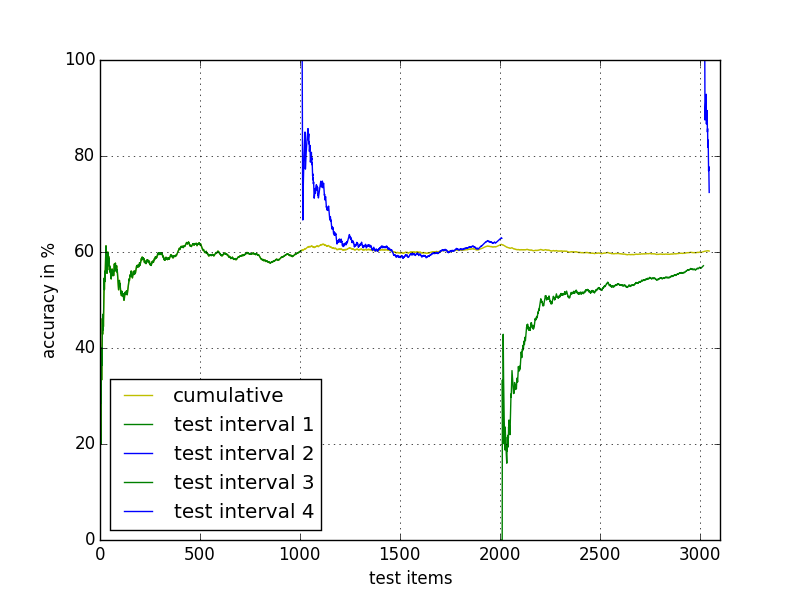
\includegraphics[width=0.2\textwidth]{./plots/batchPlot.png}\\

In the second szenario we applied the bruteforce model which rebuilt the model in the beginning of every interval.\\
   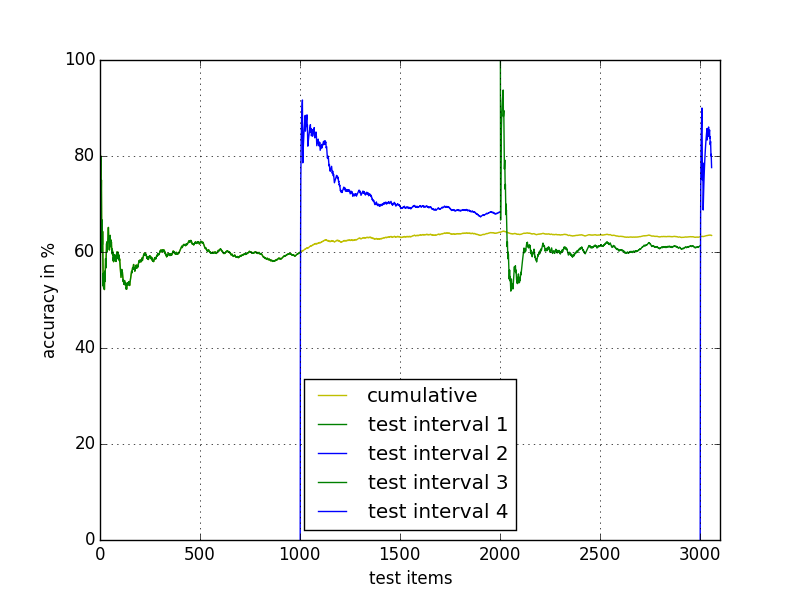
\includegraphics[width=0.2\textwidth]{./plots/bruteforce2_Plot.png}\\
In comparison with the batch version the bruteforce model gets higher accuracies in the intervals.\\

For the error-triggered model we set a threshold at 63\% of accuracy at which the model is recreated. Since we included a sanity point set the rebuilt takes place three times after the 300 sanity points and stays then constant for 1380 points after which two retraining phases follow.\\
   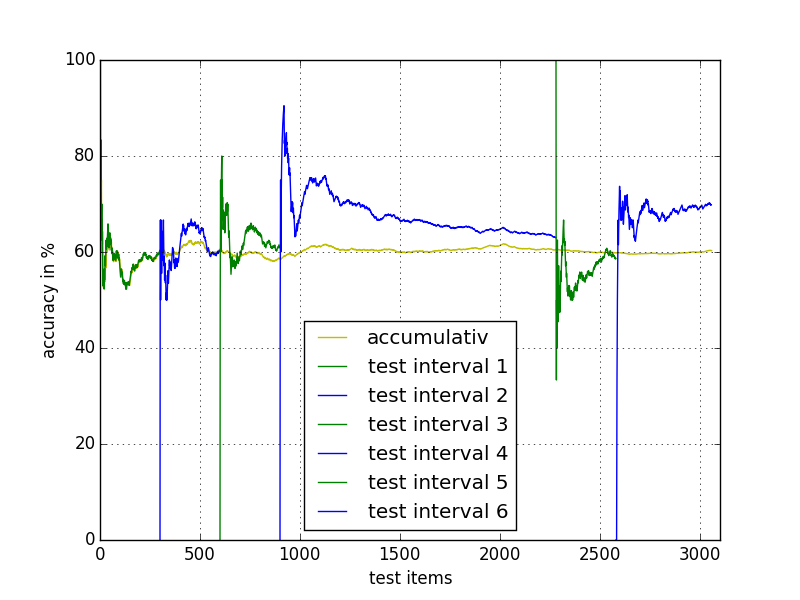
\includegraphics[width=0.2\textwidth]{./plots/errorTriggeredPlot}\\
In comparison batch and error-triggered the error-triggered has higher interval accuracy but due to the short retraining intervals avaraged they are similar. \\

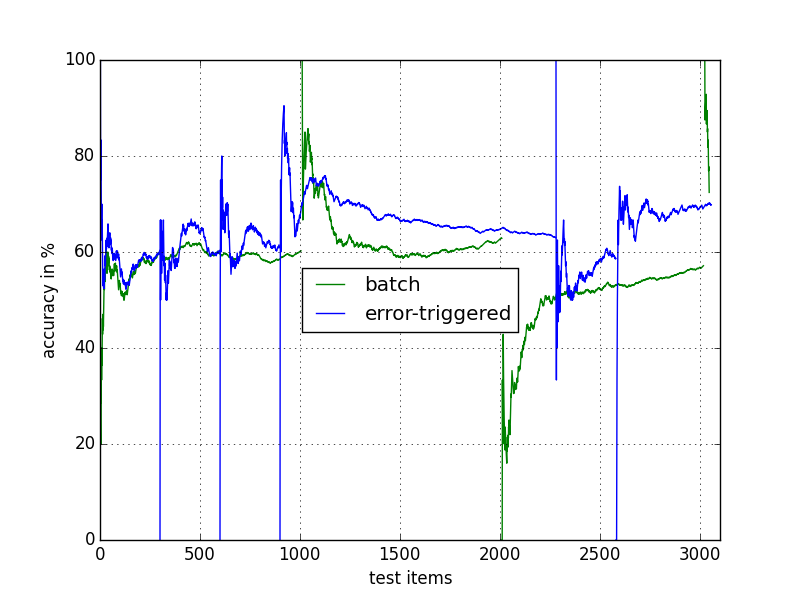
\includegraphics[width=0.2\textwidth]{./plots/errortriggered_batch}\\
Despite bruteforce and error-triggered methods have both higher interval accuracies around the phase of testpoints 1000 to 2000 which might be caused by concept drift. 
\\

The incremental one clearly outperformed all the other model-update methods although the learning rate was mostly between 0.02 and 0 except for three peak times when it is around 0.6.

   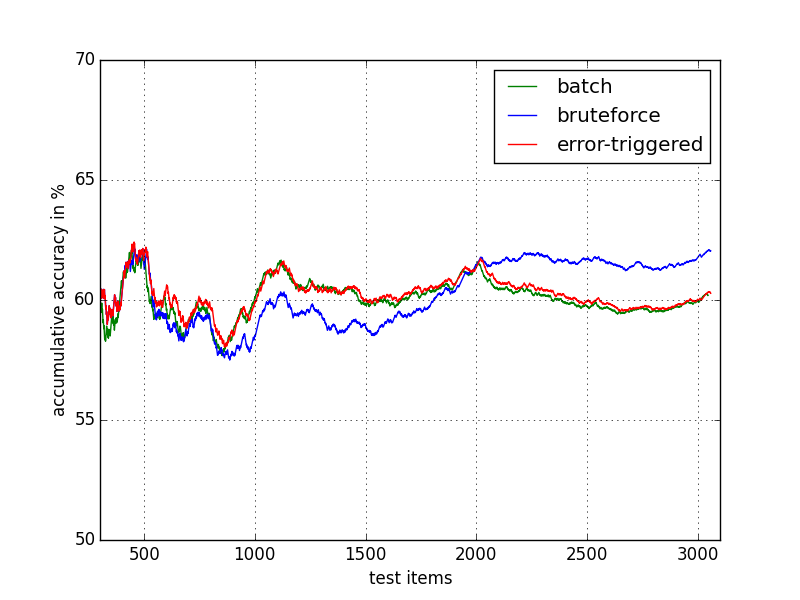
\includegraphics[width=0.2\textwidth]{./plots/allAccuracies}\\

\\
\begin{centering}
   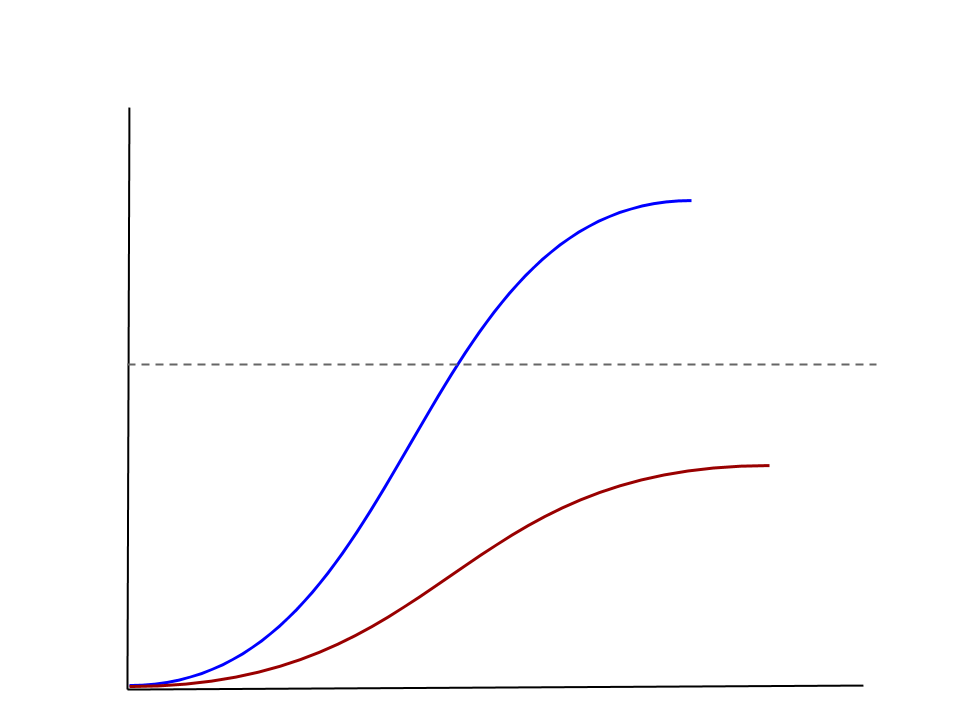
\includegraphics[width=0.2\textwidth]{./pic3}
   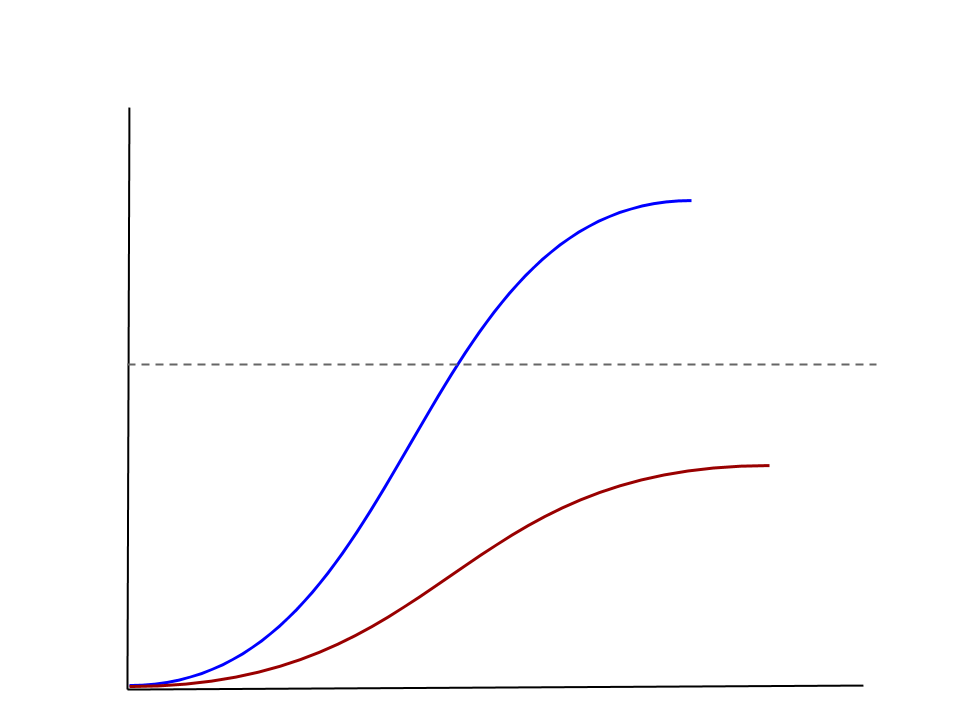
\includegraphics[width=0.2\textwidth]{./pic3}
   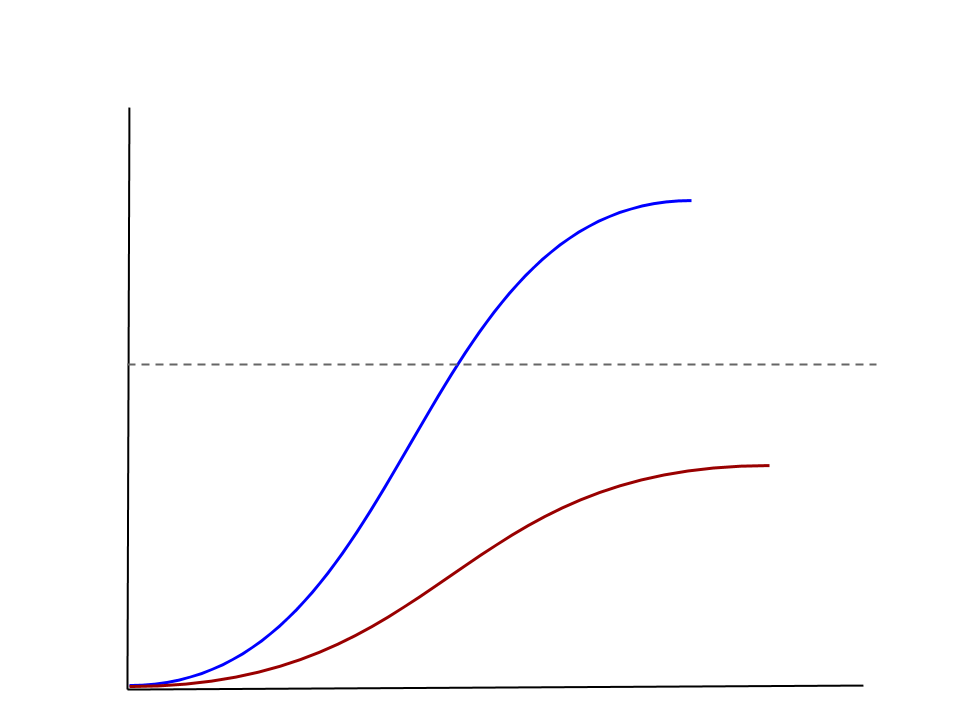
\includegraphics[width=0.2\textwidth]{./pic3}
   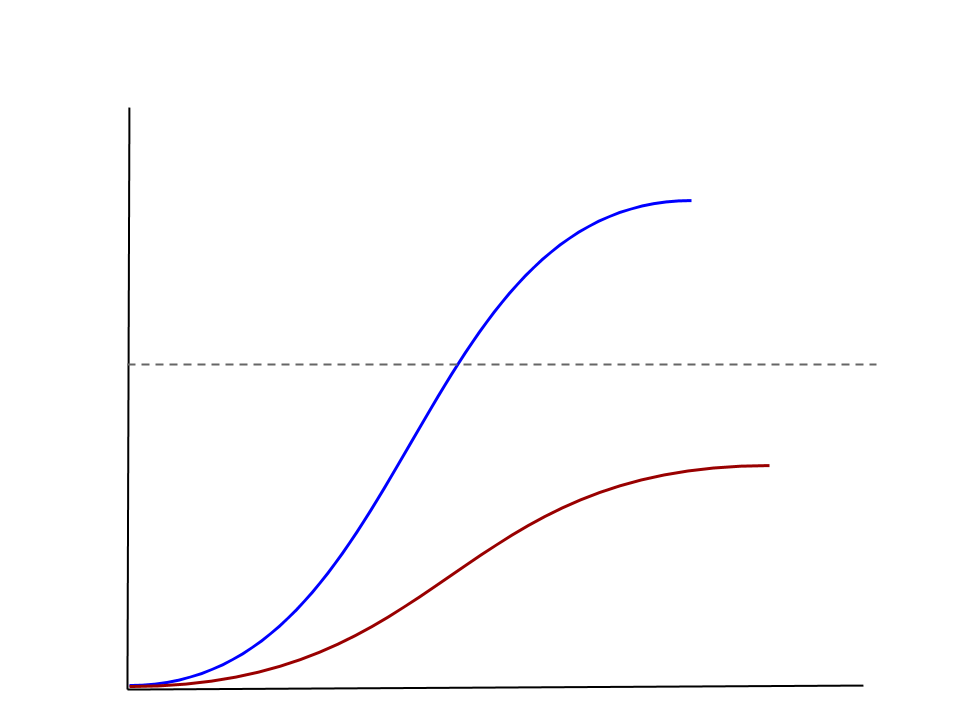
\includegraphics[width=0.2\textwidth]{./pic3}\\
\end{centering}}}

\vspace{0.8cm}
%Literature
\fcolorbox{darkgreen}{white}{\parbox{ \textwidth}{%
      \renewcommand{\baselinestretch}{1.05}\small\normalsize
\begin{thebibliography}{9} 
%\begin{left} \textbf{\huge Literature} \end{left}
\bibitem{zitat1} \textsc{C\'esar A. Astudillo and Javier I. Gonzalez}\textit{Concept Drift Detection Using Online Bayesian Classifier},Proceedings of the XXXII International Conference of The Chilean Computer Science Society, 2013.
\bibitem{zitat2} \textsc{Zaharia, Matei and Das, Tathagata and Li, Haoyuan and Shenker, Scott and Stoica, Ion}, \textit{Discretized Streams: An Efficient and Fault-tolerant Model for Stream Processing on Large Clusters}, Proceedings of the 4th USENIX Conference on Hot Topics in Cloud Computing, 2012.
\end{thebibliography}



}}
\end{document}